\documentclass{ctexart}
\usepackage{amsmath}
\usepackage{graphicx}
\usepackage{float}
\usepackage{geometry}
\usepackage{hyperref}
\usepackage{subfigure}
\usepackage{tabularx}
\title{Pictures}
\author{Qiyu Chen}
\date{\today}
\begin{document}
	\begin{figure}[H]
		\centering
		\subfigure{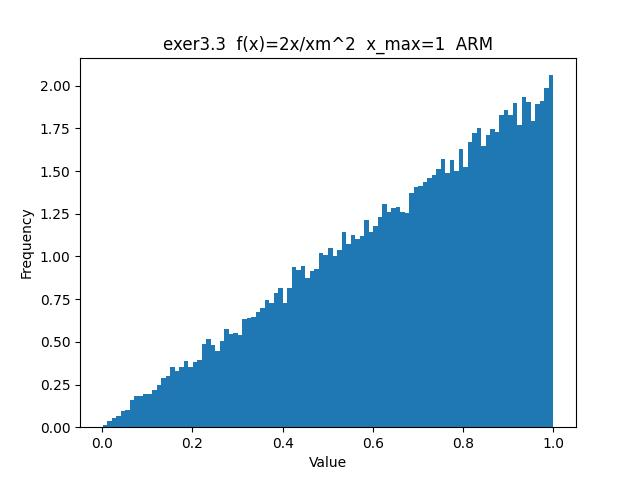
\includegraphics[width=6cm]{exer3.3_ARM.jpg}}
		\subfigure{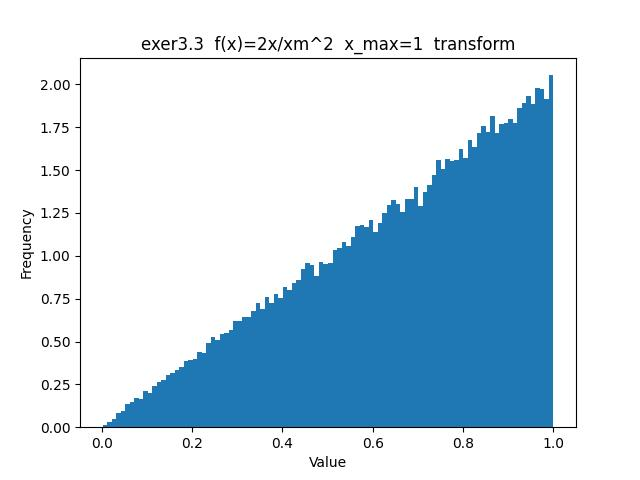
\includegraphics[width=6cm]{exer3.3_transform.jpg}}\\
	\end{figure}
	\begin{figure}[H]
		\centering
		\subfigure{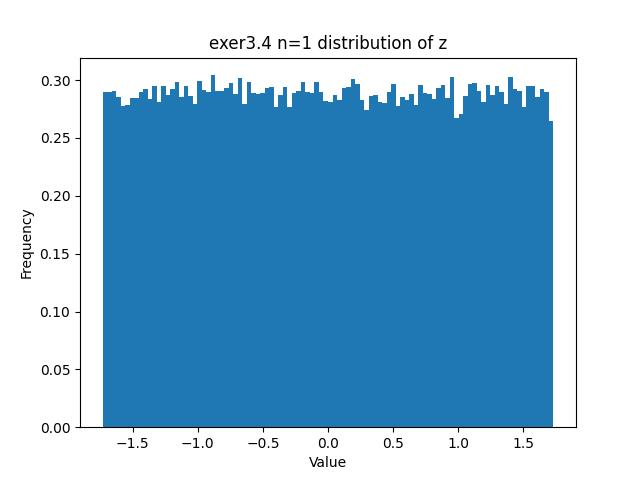
\includegraphics[width=6cm]{exer3.4_n=1.jpg}}
		\subfigure{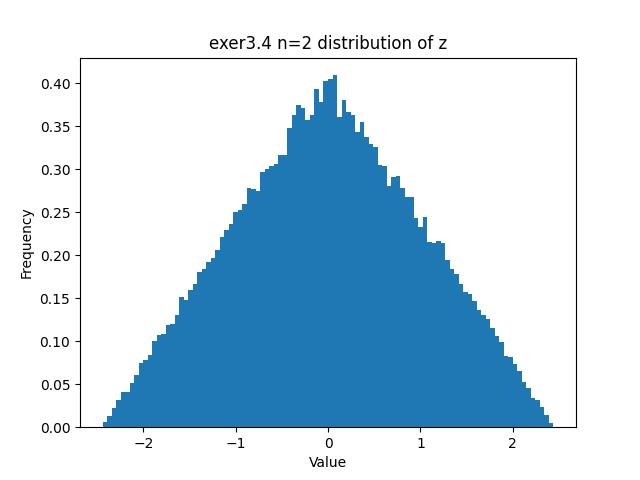
\includegraphics[width=6cm]{exer3.4_n=2.jpg}}\\
	\end{figure}
	
	\begin{figure}[H]
		\centering
		\subfigure{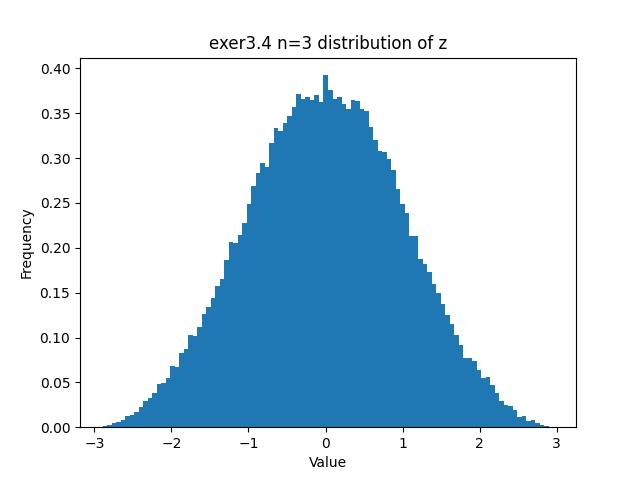
\includegraphics[width=6cm]{exer3.4_n=3.jpg}}
		\subfigure{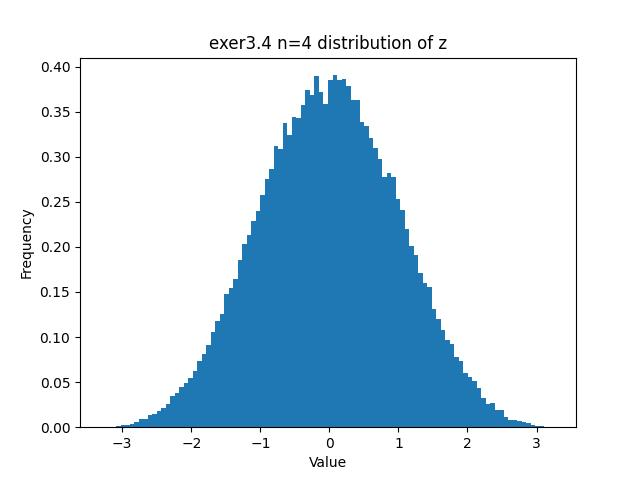
\includegraphics[width=6cm]{exer3.4_n=4.jpg}}\\
	\end{figure}
	
	\begin{figure}[H]
		\centering
		\subfigure{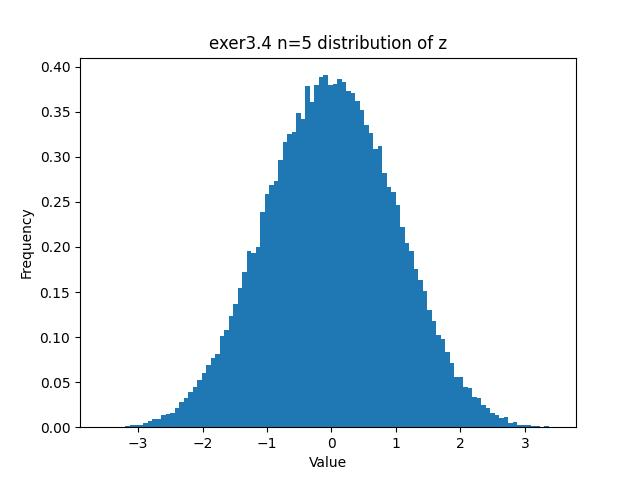
\includegraphics[width=6cm]{exer3.4_n=5.jpg}}
		\subfigure{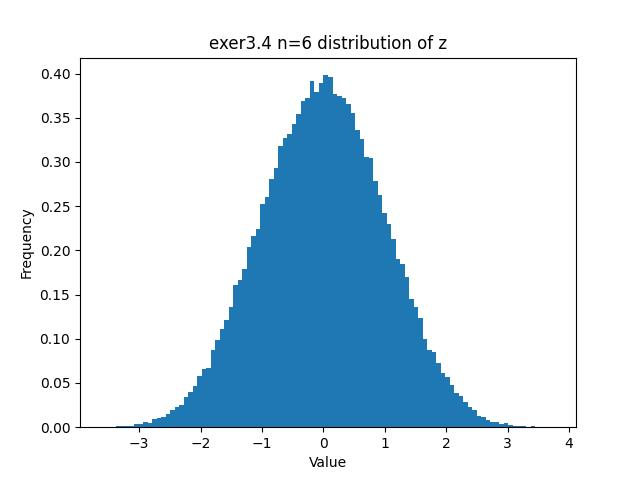
\includegraphics[width=6cm]{exer3.4_n=6.jpg}}\\
	\end{figure}
	
	\begin{figure}[H]
		\centering
		\subfigure{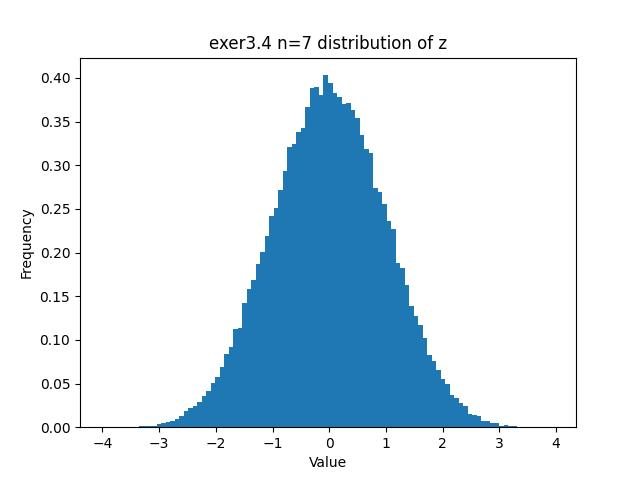
\includegraphics[width=6cm]{exer3.4_n=7.jpg}}
		\subfigure{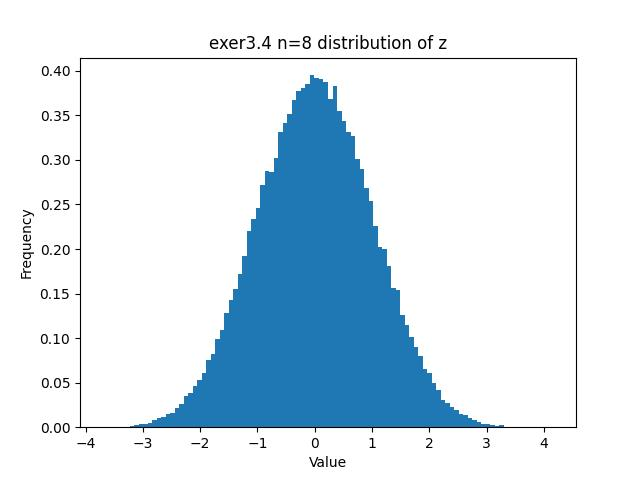
\includegraphics[width=6cm]{exer3.4_n=8.jpg}}\\
	\end{figure}
	
	\begin{figure}[H]
		\centering
		\subfigure{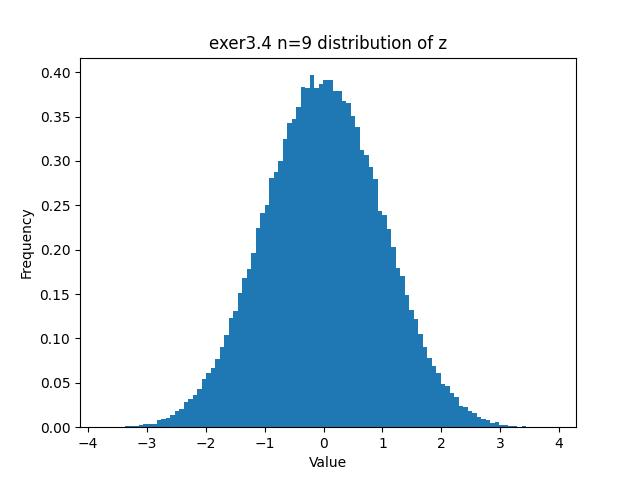
\includegraphics[width=6cm]{exer3.4_n=9.jpg}}
		\subfigure{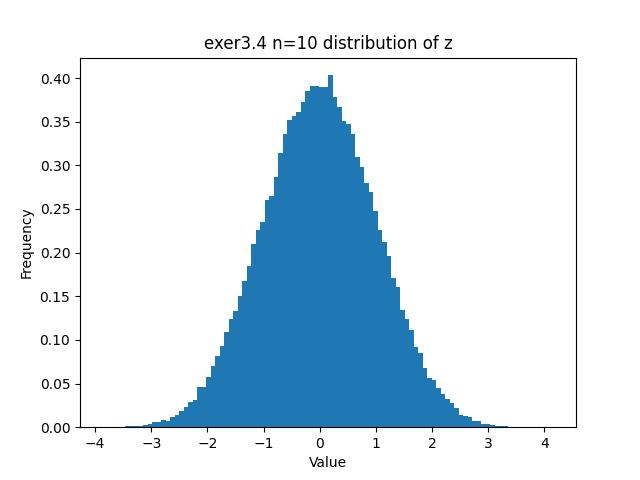
\includegraphics[width=6cm]{exer3.4_n=10.jpg}}\\
	\end{figure}
	
	\begin{figure}[H]
		\centering
		\subfigure{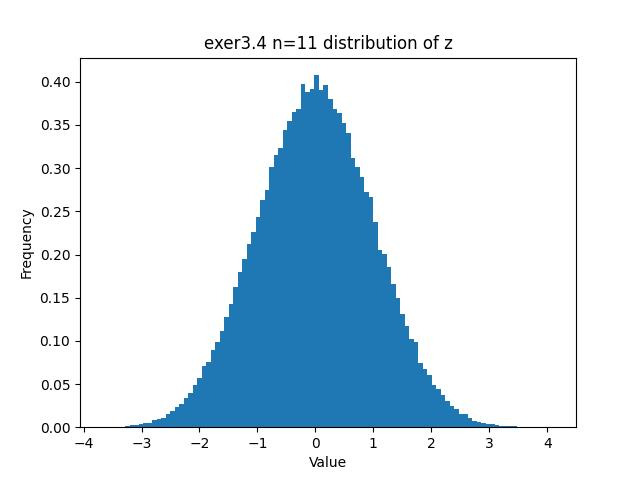
\includegraphics[width=6cm]{exer3.4_n=11.jpg}}
		\subfigure{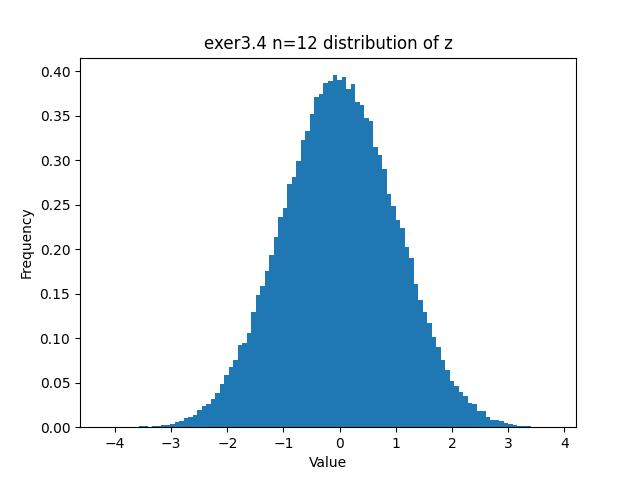
\includegraphics[width=6cm]{exer3.4_n=12.jpg}}\\
	\end{figure}
	
	\begin{figure}[H]
		\centering
		\subfigure{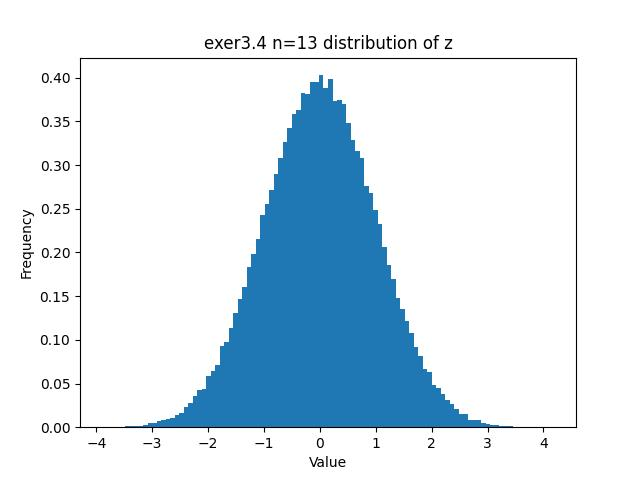
\includegraphics[width=6cm]{exer3.4_n=13.jpg}}
		\subfigure{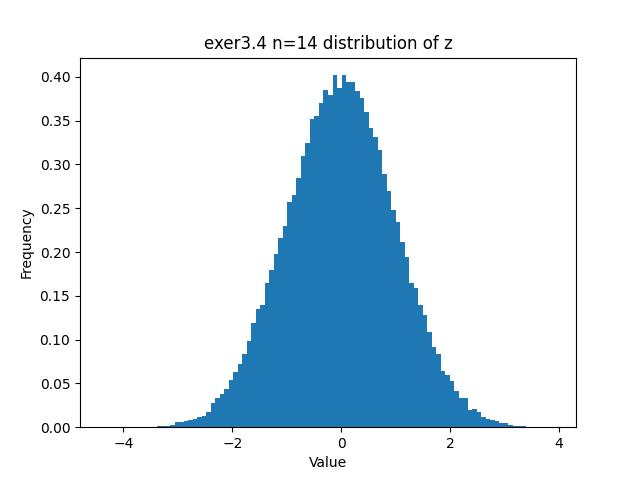
\includegraphics[width=6cm]{exer3.4_n=14.jpg}}\\
	\end{figure}
	
	\begin{figure}[H]
		\centering
		\subfigure{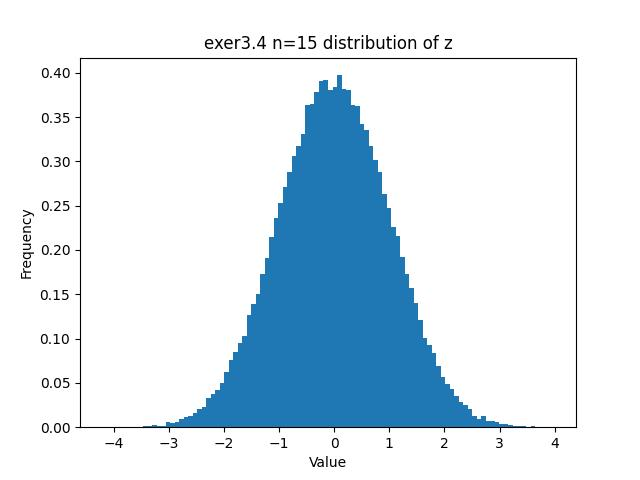
\includegraphics[width=6cm]{exer3.4_n=15.jpg}}
		\subfigure{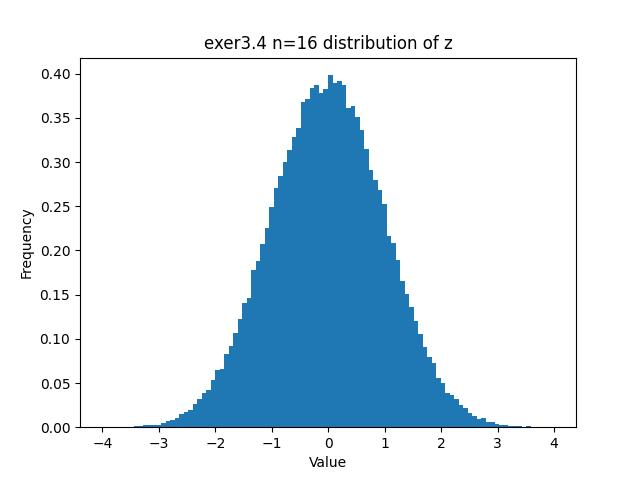
\includegraphics[width=6cm]{exer3.4_n=16.jpg}}\\
	\end{figure}
	
	\begin{figure}[H]
		\centering
		\subfigure{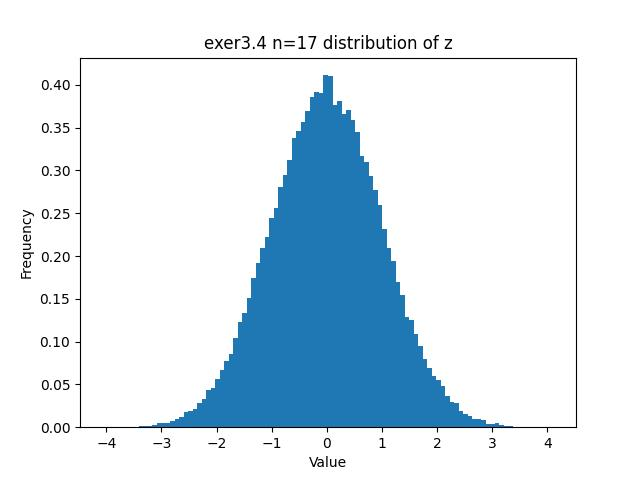
\includegraphics[width=6cm]{exer3.4_n=17.jpg}}
		\subfigure{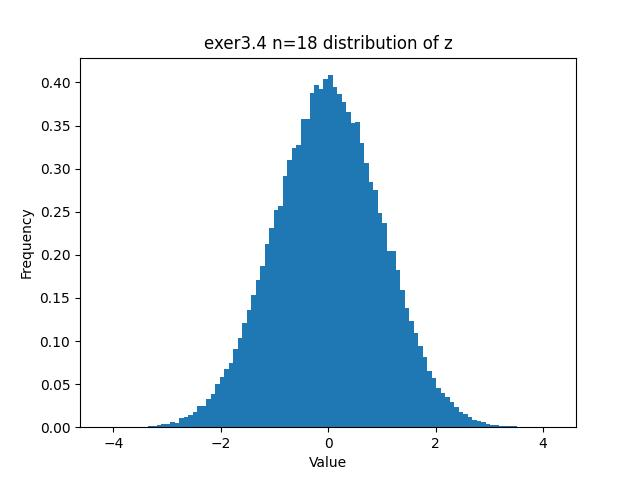
\includegraphics[width=6cm]{exer3.4_n=18.jpg}}\\
	\end{figure}
	
	\begin{figure}[H]
		\centering
		\subfigure{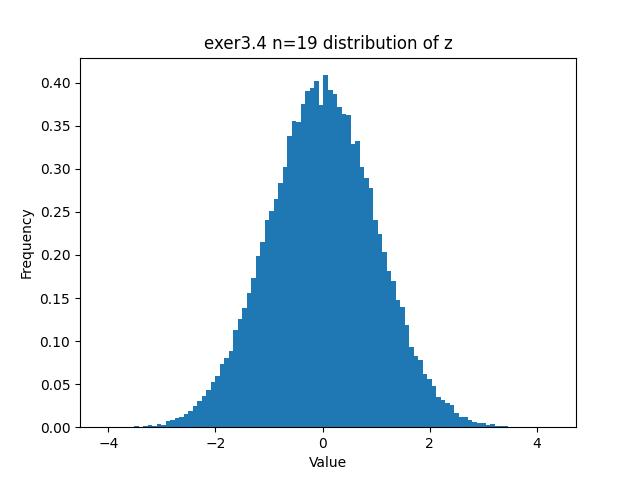
\includegraphics[width=6cm]{exer3.4_n=19.jpg}}
		\subfigure{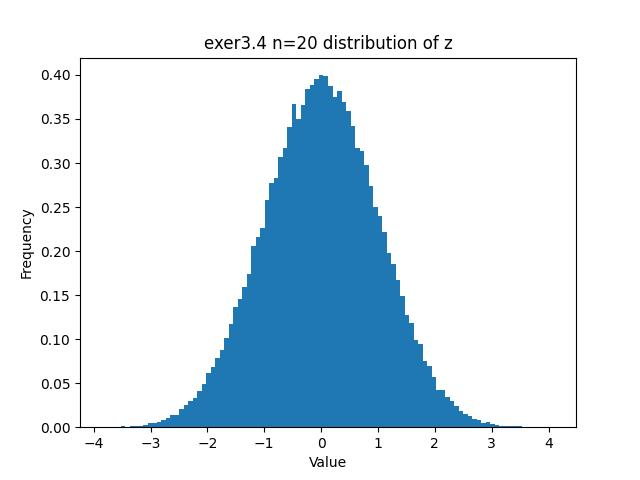
\includegraphics[width=6cm]{exer3.4_n=20.jpg}}\\
	\end{figure}
	
	\begin{figure}[H]
		\centering
		\subfigure{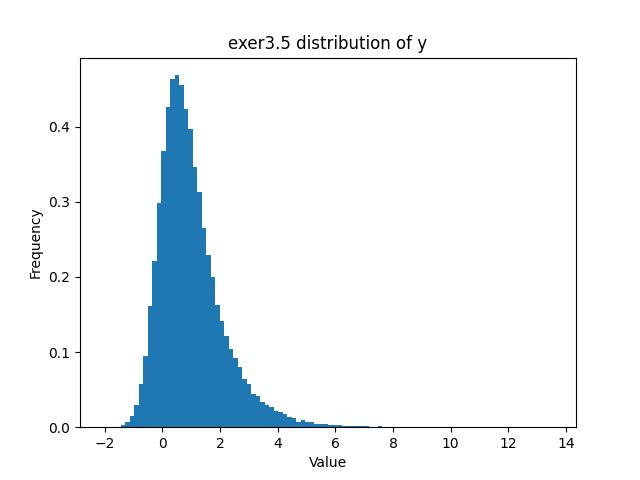
\includegraphics[width=6cm]{exer3.5.jpg}}
		\subfigure{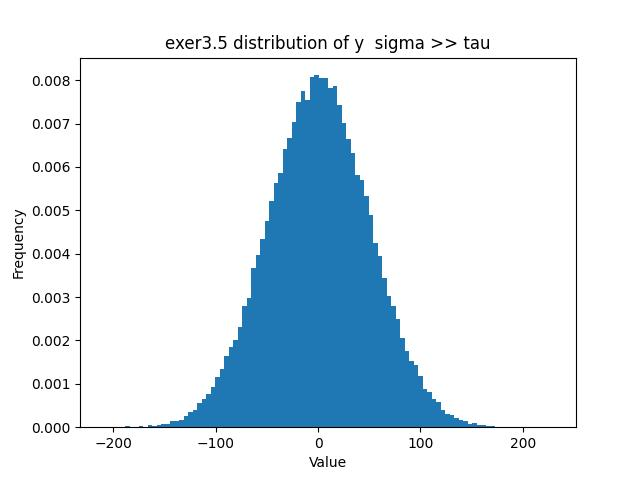
\includegraphics[width=6cm]{exer3.5_sigma_larger_than_tau.jpg}}\\
	\end{figure}
	
	\begin{figure}[H]
		\centering
		\subfigure{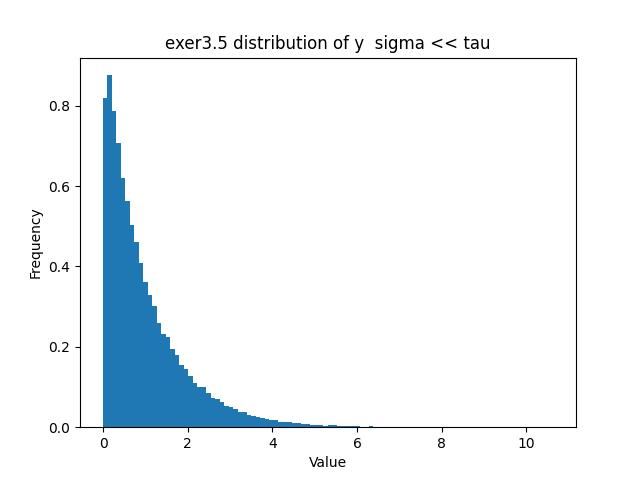
\includegraphics[width=6cm]{exer3.5_sigma_smaller_than_tau.jpg}}
		\subfigure{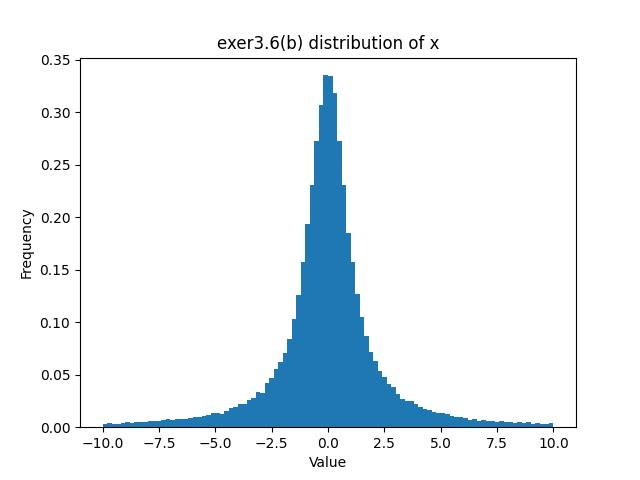
\includegraphics[width=6cm]{exer3.6(b).jpg}}\\
	\end{figure}
	
	\begin{figure}[H]
		\centering
		\subfigure{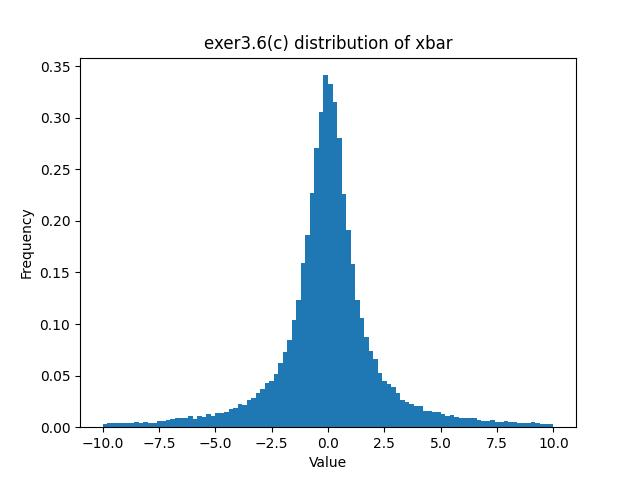
\includegraphics[width=6cm]{exer3.6(c).jpg}}
		\subfigure{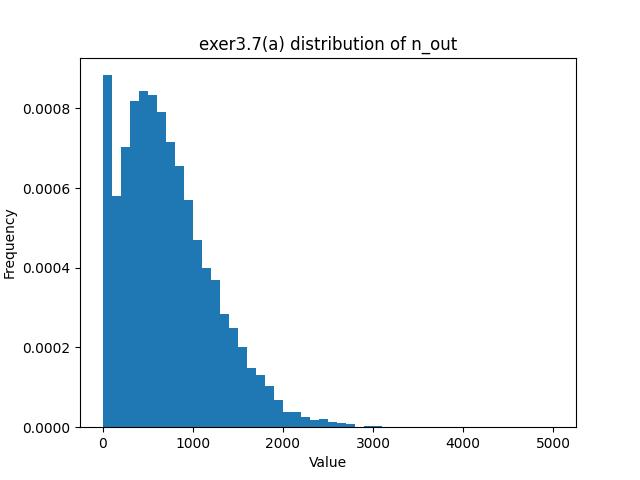
\includegraphics[width=6cm]{exer3.7(a).jpg}}\\
	\end{figure}
	
	
	\begin{figure}[H]
		\centering
		\subfigure{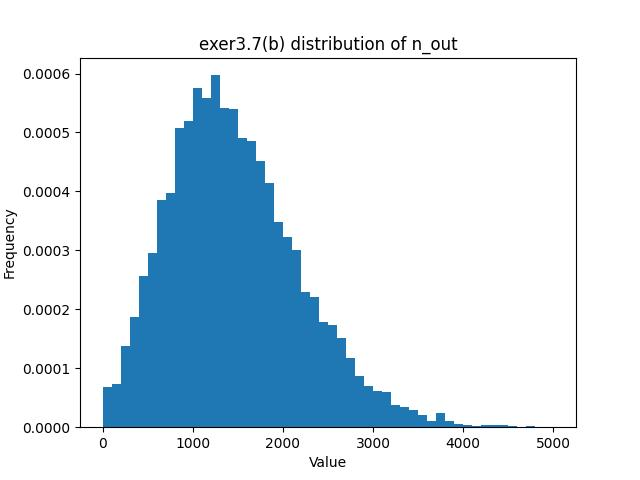
\includegraphics[width=6cm]{exer3.7(b).jpg}}
		\subfigure{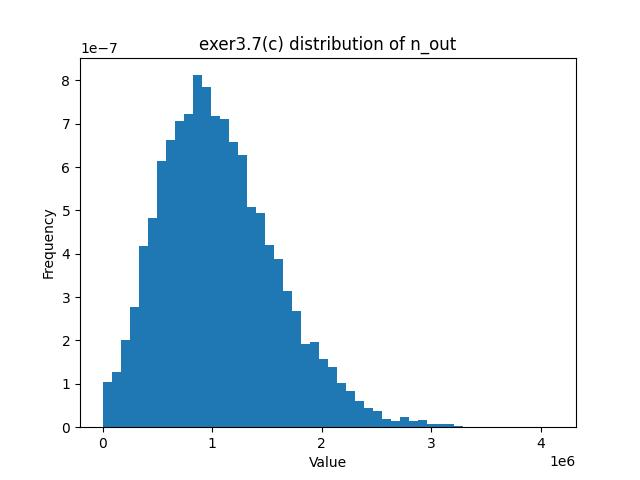
\includegraphics[width=6cm]{exer3.7(c).jpg}}\\
	\end{figure}
\end{document}